\documentclass[a4]{article}
\pagestyle{myheadings}

%%%%%%%%%%%%%%%%%%%
% Packages/Macros %
%%%%%%%%%%%%%%%%%%%
\usepackage{mathrsfs}


\usepackage{fancyhdr}
\pagestyle{fancy}
\lhead{}
\chead{}
\rhead{}
\lfoot{}
\cfoot{} 
\rfoot{\normalsize\thepage}
\renewcommand{\headrulewidth}{0pt}
\renewcommand{\footrulewidth}{0pt}
\newcommand{\RomanNumeralCaps}[1]
    {\MakeUppercase{\romannumeral #1}}

\usepackage{amssymb,latexsym}  % Standard packages
\usepackage[utf8]{inputenc}
\usepackage[russian]{babel}
\usepackage{MnSymbol}
\usepackage{mathrsfs}
\usepackage{amsmath,amsthm}
\usepackage{indentfirst}
\usepackage{graphicx}%,vmargin}
\usepackage{graphicx}
\graphicspath{{pictures/}} 
\usepackage{verbatim}
\usepackage{color}
\usepackage{color,colortbl}
\usepackage[nottoc,numbib]{tocbibind}
\usepackage{float}
\usepackage{multirow}
\usepackage{hhline}

\usepackage{listings}
\definecolor{codegreen}{rgb}{0,0.6,0}
\definecolor{codegray}{rgb}{1,1,1}
\definecolor{codepurple}{rgb}{0.58,0,0.82}
\definecolor{backcolour}{rgb}{0.95,0.95,0.92}
 
\lstdefinestyle{mystyle}{
    backgroundcolor=\color{backcolour},   
    commentstyle=\color{codegreen},
    keywordstyle=\color{magenta},
    numberstyle=\tiny\color{codegray},
    stringstyle=\color{codepurple},
    basicstyle=\footnotesize,
    breakatwhitespace=false,         
    breaklines=true,                 
    captionpos=b,                    
    keepspaces=true,                 
    numbers=left,                    
    numbersep=5pt,                  
    showspaces=false,                
    showstringspaces=false,
    showtabs=false,                  
    tabsize=2
}
 
\lstset{style=mystyle}

\usepackage{url}
\urldef\myurl\url{foo%.com}
\def\UrlBreaks{\do\/\do-}
\usepackage{breakurl}
\Urlmuskip=0mu plus 1mu



\DeclareGraphicsExtensions{.pdf,.png,.jpg}% -- настройка картинок

\usepackage{epigraph} %%% to make inspirational quotes.
\usepackage[all]{xy} %for XyPic'a
\usepackage{color} 
\usepackage{amscd} %для коммутативных диграмм
%\usepackage[colorlinks,urlcolor=red]{hyperref}

%\renewcommand{\baselinestretch}{1.5}
%\sloppy
%\usepackage{listings}
%\lstset{numbers=left}
%\setmarginsrb{2cm}{1.5cm}{1cm}{1.5cm}{0pt}{0mm}{0pt}{13mm}


\newtheorem{Lemma}{Лемма}[section]
\newtheorem{Proposition}{Предложение}[section]
\newtheorem{Theorem}{Теорема}[section]
\newtheorem{Corollary}{Следствие}[section]
\newtheorem{Remark}{Замечание}[section]
\newtheorem{Definition}{Определение}[section]
\newtheorem{Designations}{Обозначение}[section]




%%%%%%%%%%%%%%%%%%%%%%% 
%Подготовка оглавления% 
%%%%%%%%%%%%%%%%%%%%%%% 
\usepackage[titles]{tocloft}
\renewcommand{\cftdotsep}{2} %частота точек
\renewcommand\cftsecleader{\cftdotfill{\cftdotsep}}
\renewcommand{\cfttoctitlefont}{\hspace{0.38\textwidth} \LARGE\bfseries} 
\renewcommand{\cftsecaftersnum}{.}
\renewcommand{\cftsubsecaftersnum}{.}
\renewcommand{\cftbeforetoctitleskip}{-1em} 
\renewcommand{\cftaftertoctitle}{\mbox{}\hfill \\ \mbox{}\hfill{\footnotesize Стр.}\vspace{-0.5em}} 
%\renewcommand{\cftchapfont}{\normalsize\bfseries \MakeUppercase{\chaptername} } 
%\renewcommand{\cftsecfont}{\hspace{1pt}} 
\renewcommand{\cftsubsecfont}{\hspace{1pt}} 
%\renewcommand{\cftbeforechapskip}{1em} 
\renewcommand{\cftparskip}{3mm} %определяет величину отступа в оглавлении
\setcounter{tocdepth}{5} 
\renewcommand{\listoffigures}{\begingroup %добавляем номер в список иллюстраций
\tocsection
\tocfile{\listfigurename}{lof}
\endgroup}
\renewcommand{\listoftables}{\begingroup %добавляем номер в список иллюстраций
\tocsection
\tocfile{\listtablename}{lot}
\endgroup}


%\renewcommand{\thelikesection}{(\roman{likesection})}
%%%%%%%%%%%
% Margins %
%%%%%%%%%%%
\addtolength{\textwidth}{0.7in}
\textheight=630pt
\addtolength{\evensidemargin}{-0.4in}
\addtolength{\oddsidemargin}{-0.4in}
\addtolength{\topmargin}{-0.4in}

%%%%%%%%%%%%%%%%%%%%%%%%%%%%%%%%%%%
%%%%%%Переопределение chapter%%%%%% 
%%%%%%%%%%%%%%%%%%%%%%%%%%%%%%%%%%%
\newcommand{\empline}{\mbox{}\newline} 
\newcommand{\likechapterheading}[1]{ 
\begin{center} 
\textbf{\MakeUppercase{#1}} 
\end{center} 
\empline} 

%%%%%%%Запиливание переопределённого chapter в оглавление%%%%%% 
\makeatletter 
\renewcommand{\@dotsep}{2} 
\newcommand{\l@likechapter}[2]{{\bfseries\@dottedtocline{0}{0pt}{0pt}{#1}{#2}}} 
\makeatother 
\newcommand{\likechapter}[1]{ 
\likechapterheading{#1} 
\addcontentsline{toc}{likechapter}{\MakeUppercase{#1}}} 




\usepackage{xcolor}
\usepackage{hyperref}
\definecolor{linkcolor}{HTML}{000000} % цвет ссылок
\definecolor{urlcolor}{HTML}{AA1622} % цвет гиперссылок
 
\hypersetup{pdfstartview=FitH,  linkcolor=linkcolor,urlcolor=urlcolor, colorlinks=true}

%%%%%%%%%%%%
% Document %
%%%%%%%%%%%%

%%%%%%%%%%%%%%%%%%%%%%%%%%%%%
%%%%%%главы -- section*%%%%%%
%%%%section -- subsection%%%%
%subsection -- subsubsection%
%%%%%%%%%%%%%%%%%%%%%%%%%%%%%
\def \newstr {\medskip \par \noindent} 



\begin{document}
\newcolumntype{g}{>{\columncolor{codegray}}c}



\def\contentsname{\LARGE{Содержание}}
\thispagestyle{empty}
\begin{center} 
\vspace{2cm} 
{\Large \sc Санкт-Петербургский Политехнический}\\
\vspace{2mm}
{\Large \sc Университет} им. {\Large\sc Петра Великого}\\
\vspace{1cm}
{\large \sc Институт прикладной математики и механики\\ 
\vspace{0.5mm}
\textsc{}}\\ 
\vspace{0.5mm}
{\large\sc Кафедра прикладной математики}\\
\vspace{15mm}
%\rule[0.5ex]{\linewidth}{2pt}\vspace*{-\baselineskip}\vspace*{3.2pt} 
%\rule[0.5ex]{\linewidth}{1pt}\\[\baselineskip] 
{\huge \sc Сводный отчёт по дисциплине "Математическая статистика" по лабораторным отчётам $5-8$\\
\vspace{6mm}
 }
\vspace*{2mm}
%\rule[0.7ex]{\linewidth}{1pt}\vspace*{-\baselineskip}\vspace{3.2pt} 
%\rule[0.5ex]{\linewidth}{2pt}\\ 
\vspace{1cm}

{\sc $3$ курс$,$ группа $33631/2$}

\vspace{2cm} 
Студент \hfill Д. А. Плаксин\\
\vspace{1cm}
Преподаватель \hfill Баженов А. Н.\\
\vspace{20mm} 

\end{center} 
%\author{Я}
\begin{center}
\vfill {\large\textsc{Санкт-Петербург}}\\ 
2019 г.
\end{center}

%%%%%%%%%%%%%%%%%%%%%%%%%%%%%%%%%%%%%%%%%%%%%%%%%%%%%%%%%%%%%%%%%%%%%%%%%%%%%%%%%%%%%%%%%%%%%%
%\ \\[4cm]

%\rm
%%%%%%%%%%%%%%%%%%%%%%%%%%%%%%%%%%%%%%%%%%%%%%%%%%%%%%%%%%%%%%%%%%%%%%%%%%%%%%%%%%%%%%%%%%%%%%
\newpage
\pagestyle{plain}

%\begin{center}
%\begin{abstract} 

%\end{abstract}

%\end{center}

\newpage
\tableofcontents{}
\newpage
\listoffigures{}
\listoftables{}
\newpage

\section{Постановка задачи}

\subsection{Вычисление коэффициента корреляции}

Необходимо построить выборки объёмом $20, 60, 100, 1000$ для двумерного нормального распределения с коэффициентами корреляции $\rho = 0, 0.5, 0.9$

Вычислить коэффициент корреляции Пирсона, Спирмана и квадрантный коэффициент корреляции для каждой выборки. Эти же вычисления повторить для смеси двумерных нормальных распределений \cite{mix}: 
\begin{equation}
    f(x,y) = 0.9N(x,y,0,0,1,1,0.9)+0.1N(x,y,0,0,10,10,-0.9)
\end{equation}
На графике изобразить точки выборки и эллипс равновероятности.

\subsection{Оценки линий регрессии}
Необходимо найти оценки линейной регрессии $y_i=a+bx_i+e_i,$ используя $20$ точек отрезка $[-1.8;\;2]$ с равномерным шагом $0.2.$ Ошибку $e_i$ считать нормально распределённой с параметрами $(0,\;1).$ В качестве эталонной зависимости взять $y_i=2+2x_i+e_i.$ При построении оценок коэффициентов использовать два критерия: критерий наименьших квадратов и критерий наименьших модулей.

\subsection{Точечная оценка параметров распределения}

Необходимо сгенерировать выборку объемом $100$ элементов для нормального распределения $N(x;0,1).$ По сгенерированной выборке оценить параметры $\mu$ и $\sigma$ нормального закона методом максимального правдоподобия. В качестве основной гипотезы $H_0$ будем считать, что сгенерированное распределение имеет вид $N(x,\overset{\wedge}{\mu},\overset{\wedge}{\sigma} ).$ Проверить основную гипотезу, используя критерий согласия $\chi$. В качестве ровня значимости взять $\alpha=0,05.$ Привести таблицу вычислений $\chi^2.$
\subsection{Интервальные оценки параметров распределения}

Для двух выборок $20$ и $100$ элементов, сгенерированных согласно нормальному закону $N(x,0,1),$ для параметров масштаба и положения построить асимптотически нормальные интервальные оценки на основе точечных оценок метода максимального правдоподобия и классические интервальные оценки на основе статистик $\chi^2$ и Стьюдента. В качестве параметра надёжности взять $\gamma = 0.95.$




\section{Теория}

\subsection{Вычисление коэффициента корреляции}

\begin{enumerate}
    \item Двумерное нормально распределение \cite{5_1}:
        \begin{equation}
        N(x,y,0,0,1,1,\rho) = \frac{1}{2\pi\sqrt{1-\rho^2}}e^{-\frac{1}{2(1-\rho^2)}(x^2-2\rho x y+y^2)} \label{dnd}
        \end{equation}
    
    \item Коэффициент корреляции Пирсона \cite{5_2}:
        \begin{equation}
        r_{xy} = \left(\sum\limits_{i=1}^n(x_i-\overline{x})(y_i-\overline{y})\right)\left(\sum\limits_{i=1}^n(x_i-\overline{x})^2\sum\limits_{i=1}^n(y_i-\overline{y})^2\right)^{-\frac{1}{2}} \label{ccp}
        \end{equation}
    \item Коэффициент корреляции Спирмана \cite{5_3}:
        \begin{equation}
        \rho_n = 1 -  \frac{6}{n^3-n}\sum\limits_{i=1}^n d_i^2\label{ccs}
        \end{equation}
        
    \item Квадрантный коэффициент корреляции \cite{5_4}:
        \begin{equation}
        \overset{\wedge}{q} = \frac{1}{n}\sum\limits_{i=1}^n sign(x_i-med\;x)sign(y_i-med\;y)\label{qcc}
        \end{equation}
\end{enumerate}

\subsection{Оценки линий регрессии}
Простая линейная регрессия \cite{lin_reg}:
\begin{equation}
    y_i=ax_i+b+e_i,\;i=\overline{1,n},\hfill
\end{equation}

где $x_i\;\--$ заданные числа, $y_i\;\--$ наблюдаемые значения, $e_i\;\--$ независимы и нормально распределены, $a$ и $b\;\--$ неизвестные параметры, подлежащие оцениванию.

\subsubsection{Метод наименьших квадратов}

Критерий $\--$ минимизация функции \cite{MNK}:
\begin{equation}
    Q(a,b)=\sum\limits_{i=1}^n(y_i-ax_i-b)^2\to \min\hfill
\end{equation}

Оценка $\overset{\wedge}{a}$ и $\overset{\wedge}{b}$ параметров $a$ и $b,$ в которых достигается минимум $Q(a,b),$ называются МНК-оценками. В случае линейной регрессии их можно вычислить из формулы \cite{6_3}:
\begin{equation}
    \begin{cases}
    \overset{\wedge}{a} = \frac{\overline{x y}-\overline{x}\overline{y}}{\overline{x^2}-\overline{x}^2}\\
    \overset{\wedge}{b} = \overline{y}-\overset{\wedge}{a}\overline{x}
    \end{cases}\hfill
\end{equation}

Метод наименьших квадратов является несмещённой оценкой.

МНК чувствителен к выбросам (т.к. в вычислении используется выборочное среднее значение величин крайне неустойчивое к редким и большим по величине выбросам)

\subsubsection{Метод наименьших модулей}
Критерий наименьших модулей – заключается в минимизации следующей функции \cite{6_4}:
\begin{equation}
    M(a,b) = \sum\limits_{i=1}^n\vert y_i-ax_i-b\vert\to\min\hfill
\end{equation}

МНМ-оценки обладают свойством робастности
Но на практике решение реализуется только численно

\subsection{Точечная оценка параметров распределения}
\subsubsection{Метод максимального правдоподобия}
Метод максимального правдоподобия $\--$ метод оценивания неизвестного параметра путём максимимзации функции правдоподобия.
\begin{equation}
    \overset{\wedge}{\theta}_{\text{МП}}=argmax \mathbf{L}(x_1,x_2,\ldots,x_n,\theta)
\end{equation}

Где $\mathbf{L}$ это функция правдоподобия, которая представляет собой совместную плотность вероятности независимых случайных величин $X_1,x_2,\ldots,x_n$ и является функцией неизвестного параметра $\theta$
\begin{equation}
    \mathbf{L} = f(x_1,\theta)\cdot f(x_2,\theta)\cdot\cdots\cdot f(x_n,\theta)
\end{equation}
Оценкой максимального правдоподобия будем называть такое значение $\overset{\wedge}{\theta}_{\text{МП}}$ из множества допустимых значений параметра $\theta,$ для которого функция правдоподобия принимает максимальное значение при заданных $x_1,x_2,\ldots,x_n.$

Тогда при оценивании математического ожидания $m$ и дисперсии $\sigma^2$ нормального распределения $N(m,\sigma)$ получим:
\begin{equation}
    \ln(\mathbf{L})=-\frac{n}{2}\ln(2\pi)-\frac{n}{2}\ln\left(\sigma^2\right)-\frac{1}{2\sigma^2}\sum\limits_{i=1}^n(x_i-m)^2
\end{equation}

\subsubsection{Критерий согласия Пирсона}
Разобьём генеральную совокупность на $k$ неперсекающихся подмножеств $\Delta_1, \Delta_2,\ldots, \Delta_k,\;\Delta_i = (a_i,a_{i+1}],$ $p_i = P(X\in\Delta_i),\;i=1,2,\ldots,k\; \--$ вероятность того, что точка попала в $i$ый промежуток.

Так как генеральная совокупность это $\mathbb{R},$ то крайние промежутки будут бесконечными: $\Delta_1=(-\infty,a_1],\;\Delta_k=(a_k,\infty),\;p_i = F(a_i)-F(a_{i-1})$

$n_i\;\--$ частота попадания выборочных элементов в $\Delta_i,\;i=1,2,\ldots,k.$

В случае справедливости гипотезы $H_0$ относительно частоты $\frac{n_i}{n}$ при больших $n$ должны быть близки к $p_i,$ значит в качестве меры имеет смысл взять: 
\begin{equation}
    Z = \sum\limits_{i=1}^k\frac{n}{p_i}\left(\frac{n_i}{n}-p_i\right)^2
\end{equation}
Тогда
\begin{equation}
    \chi^2_B=\sum\limits_{i=1}^k\frac{n}{p_i}\left(\frac{n_i}{n}-p_i\right)^2=\sum\limits_{i=1}^k\frac{(n_i-np_i)^2}{np_i}
\end{equation}
Для выполнения гипотезы $H_0$ должны выполняться следующие условия \cite{7_2}:
\begin{equation}
    \chi_B^2 < \chi_{1-\alpha}^2(k-1)
\end{equation}
где $\chi_{1-\alpha}^2(k-1)\;\--$ квантиль распределения $\chi^2$ с $k-1$ степенями свободы порядка $1-\alpha,$ где $\alpha$ заданный уровень значимости.

\subsection{Интервальные оценки параметров распределения}

Оценкой максимального правдоподобия для математического ожидания  является среднее арифметическое: $\mu=\frac{1}{n}\sum\limits_{i=1}^nx_i.$

Оценка максимального правдоподобия для дисперсии вычисляется по формуле: $\sigma^2 = \frac{1}{n}\sum\limits_{i=1}^n(x_i-\overline{x})^2.$

Доверительным интервалом или интервальной оценкой числовой характеристики или параметра распределения $\theta$ с доверительной вероятностью $\gamma$ называется интервал со случайными границами $(\theta_1,\theta_2),$ содержащий параметр $\theta$ с вероятностью $\gamma$ \cite{8_1}.

Функция распределения Стьюдента \cite{8_2}:
\begin{equation}
    T = \sqrt{n-1}\frac{\overline{x}-\mu}{\delta}
\end{equation}

Функция плотности распределения $\chi^2$ \cite{8_3}:
\begin{equation}
    f(x) = \begin{cases}
    0,&x\leq 0\\
    \frac{1}{2^\frac{n}{2}\Gamma\left(\frac{n}{2}\right)}x^{\frac{n}{2}-1}e^{-\frac{x}{2}},& x>0
    \end{cases}
\end{equation}

Интервальная оценка математического ожидания \cite{8_4}:
\begin{equation}
    P=\left(\overline{x}-\frac{\sigma t_{1-\frac{a}{2}}(n-1)}{\sqrt{n-1}}<\mu<\overline{x}+\frac{\sigma t_{1-\frac{a}{2}}(n-1)}{\sqrt{n-1}}\right) = \gamma,
\end{equation}
где $t_{1-\frac{a}{2}}\;\--$ квантиль распределения Стьюдента порядка $1-\frac{a}{2}.$

Интервальная оценка дисперсии \cite{8_2}:
\begin{equation}
    P=\left(\frac{\sigma\sqrt{n}}{\sqrt{\chi^2_{1-\frac{a}{2}}(n-1)}}<\sigma<\frac{\sigma\sqrt{n}}{\sqrt{\chi^2_\frac{a}{2}(n-1)}}\right) = \gamma,
\end{equation}
где $\chi_{1-\frac{a}{2}}^2,\;\chi_\frac{a}{2}^2\;\--$ квантили распределения Стьюдента порядков $1-\frac{a}{2}$ и $\frac{a}{2}$ соответственно.

Асимптотическая интервальная оценка математического ожидания \cite{8_2}:
\begin{equation}
    P = \left(\overline{x}-\frac{\sigma u_{1-\frac{a}{2}}}{\sqrt{n}}<\mu<\overline{x}+\frac{\sigma u_{1-\frac{a}{2}}}{\sqrt{n}}\right)=\gamma,
\end{equation}
где $u_{1-\frac{a}{2}}\;\--$ квантиль нормального распределения $N(x,0,1)$ порядка $1-\frac{a}{2}.$

\section{Реализация}
Работы была выполнена на языке $Python 3.7.$
Для генерации выборок использовался модуль \cite{numpy}.
Для построения графиков использовалась библиотека matplotlib \cite{plotlib}.
Функции распределения обрабатывались при помощи библиотеки scipy.stats \cite{skp}

\section{Результаты}
\subsection{Вычисление коэффициента корреляции}
%\vspace{-2cm}
\begin{figure}[H]
    \centering
    \caption{Графики двумерного нормального распределения\eqref{dnd} при $p=0.0$ }
    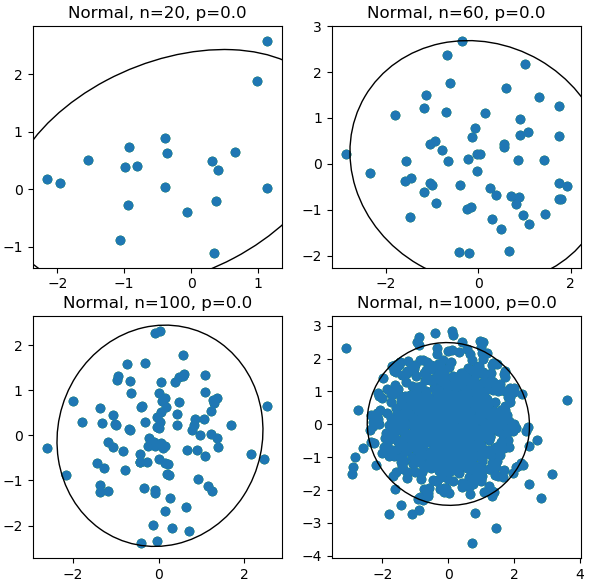
\includegraphics[scale = 0.8]{dotsNormal.png} 
    \label{fig:dis_norm_gis0}
\end{figure}
\begin{table}[H]
\caption{Результаты для двумерного нормального распределения \eqref{dnd} при $p=0.0$}
\label{tab:my_label1_1}
\begin{center}
\vspace{5mm}
\begin{tabular}{|c|c|c|c|g|c|c|c|c|}
\hhline{----~----}
\multicolumn{4}{|c|}{Normal  $n=20,\;  p=0.0$} &\multirow{11}{*}{$\cdot$} & \multicolumn{4}{c|} {Normal  $n=60,\;  p=0.0$}
\\
\hhline{----~----}
&Pearson     &Spearman    &Quad &   & & Pearson     &Spearman    &Quad        \\    
\hhline{----~----}
		E   &$0.18892$&0.14541&0.06000&  &E   &-0.04642&-0.05109&-0.03333\\
\hhline{----~----}
		$E^2$ &0.05409&0.04186&0.02800&  &$E^2$ &0.01080&0.00965&0.00667\\
\hhline{----~----}
		D   &0.01840&0.02071&0.02440&  &D   &0.00865&0.00704&0.00556\\\rowcolor{codegray}
\hhline{----~----} 
\multicolumn{9}{c}{}\\
\hhline{----~----}
\multicolumn{4}{|c|}{Normal  $n=100,\;  p=0.0$} & & \multicolumn{4}{c|}{Normal  $n=1000,\;  p=0.0$}\\
\hhline{----~----}
&Pearson     &Spearman    &Quad&  & &Pearson     &Spearman    &Quad     \\
\hhline{----~----}
		E   &-0.03469&-0.02805&-0.03200& &E   &0.00805&0.01039&0.00760\\
\hhline{----~----}
		$E^2$ &0.00531&0.00539&0.00864& &$E^2$ &0.00094&0.00083&0.00094\\
\hhline{----~----}
		D   &0.00411&0.00461&0.00762& &D   &0.00088&0.00073&0.00088\\
\hhline{----~----}
\end{tabular}
\end{center}
\end{table}




\vspace{-10cm}
\begin{figure}[H]
    \centering
    \caption{Графики двумерного нормального распределения\eqref{dnd} при $p=0.5$ }
    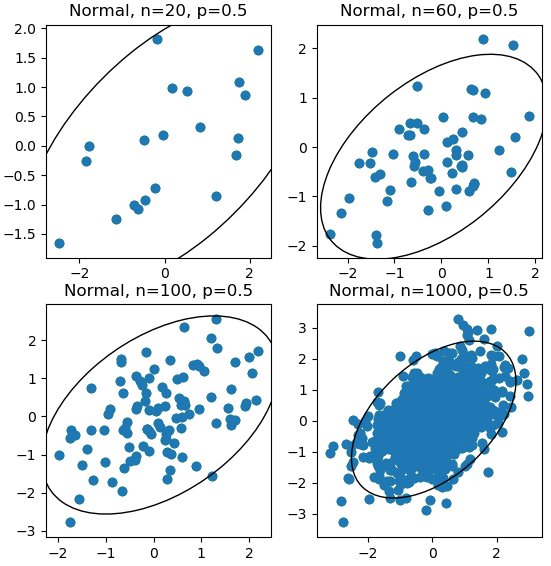
\includegraphics{dotsNormal1.png}
    \label{fig:dis_norm_gis1}
\end{figure}
\begin{table}[H]
\caption{Результаты для двумерного нормального распределения \eqref{dnd} при $p=0.5$}
\label{tab:my_label1_2}
\begin{center}
\vspace{5mm}
\begin{tabular}{|c|c|c|c|g|c|c|c|c|}
\hhline{----~----}
\multicolumn{4}{|c|}{Normal  $n=20,\;  p=0.5$} &\multirow{11}{*}{$\cdot$} & \multicolumn{4}{c|} {Normal  $n=60,\;  p=0.5$}
\\
\hhline{----~----}
&Pearson     &Spearman    &Quad &   & & Pearson     &Spearman    &Quad        \\    
\hhline{----~----}
		E   &0.50363&0.52647&0.46000&  &E   &0.50847&0.47194&0.31333\\
\hhline{----~----}
		$E^2$ &0.27217&0.30152&0.22800&  &$E^2$ &0.26921&0.23710&0.12222\\
\hhline{----~----}
		D   &0.01853&0.02435&0.01640&  &D   &0.01067&0.01437&0.02404\\\rowcolor{codegray}
\hhline{----~----} 
\multicolumn{9}{c}{}\\
\hhline{----~----}
\multicolumn{4}{|c|}{Normal  $n=100,\;  p=0.5$} & & \multicolumn{4}{c|}{Normal  $n=1000,\;  p=0.5$}\\
\hhline{----~----}
&Pearson     &Spearman    &Quad&  & &Pearson     &Spearman    &Quad     \\
\hhline{----~----}
		E   &0.49628&0.47702&0.33200& &E   &0.49458&0.47938&0.33320\\
\hhline{----~----}
		$E^2$ &0.25200&0.23489&0.12048& &$E^2$ &0.24515&0.23052&0.11207\\
\hhline{----~----}
		D   &0.00570&0.00734&0.01026& &D   &0.00054&0.00071&0.00105\\
\hhline{----~----}
\end{tabular}
\end{center}
\end{table}



\vspace{-1cm}
\begin{figure}[H]
    \centering
    \caption{График двумерного нормального распределения \eqref{dnd} при $p=0.9$ }
    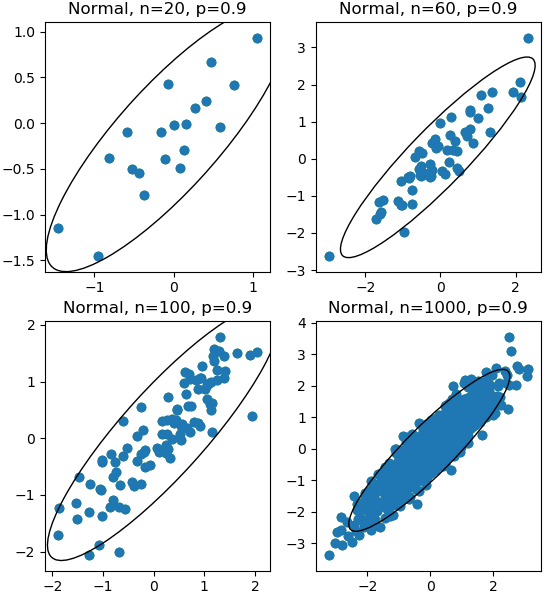
\includegraphics{dotsNormal2.png} 
    \label{fig:dis_norm_gis2}
\end{figure}
\begin{table}[H]
\caption{Результаты для двумерного нормального распределения \eqref{dnd} при $p=0.9$}
\label{tab:my_label3}
\begin{center}
\vspace{5mm}
\begin{tabular}{|c|c|c|c|g|c|c|c|c|}
\hhline{----~----}
\multicolumn{4}{|c|}{Normal  $n=20,\;  p=0.9$} &\multirow{11}{*}{$\cdot$} & \multicolumn{4}{c|} {Normal  $n=60,\;  p=0.9$}
\\
\hhline{----~----}
&Pearson     &Spearman    &Quad &   & & Pearson     &Spearman    &Quad        \\    
\hhline{----~----}
		E   &0.90154&0.85850&0.64000&  &E   &0.89761&0.88464&0.69333\\
\hhline{----~----}
		$E^2$ &0.81558&0.74275&0.44000&  &$E^2$ &0.80681&0.78457&0.48622\\
\hhline{----~----}
		D   &0.00281&0.00574&0.03040&  &D   &0.00112&0.00198&0.00551\\\rowcolor{codegray}
\hhline{----~----} 
\multicolumn{9}{c}{}\\
\hhline{----~----}
\multicolumn{4}{|c|}{Normal  $n=100,\;  p=0.9$} & & \multicolumn{4}{c|}{Normal  $n=1000,\;  p=0.9$}\\
\hhline{----~----}
&Pearson     &Spearman    &Quad&  & &Pearson     &Spearman    &Quad     \\
\hhline{----~----}
		E   &0.89624&0.88888&0.71600& &E   &0.89971&0.88953&0.71120\\
\hhline{----~----}
		$E^2$ &0.80360&0.79094&0.51728& &$E^2$ &0.80951&0.79132&0.50603\\
\hhline{----~----}
		D   &0.00037&0.00082&0.00462& &D   &0.00004&0.00005&0.00022\\
\hhline{----~----}
\end{tabular}
\end{center}
\end{table}





\vspace{-1cm}
\begin{figure}[H]
    \centering
    \caption{Графики смеси двумерных нормальных распределений }
    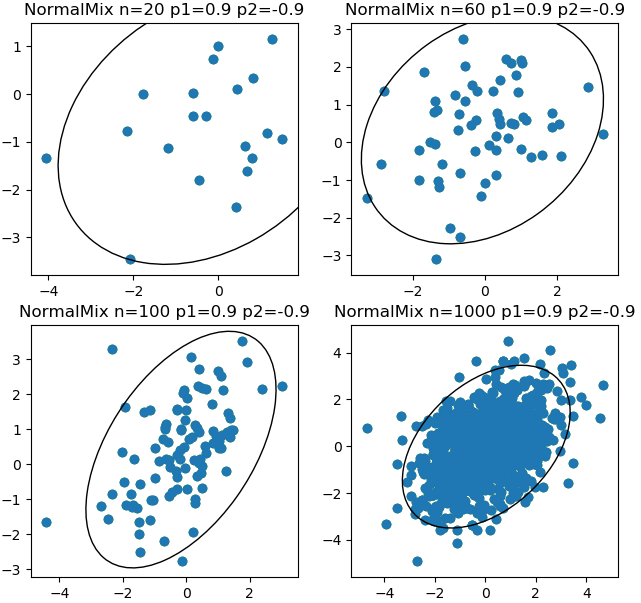
\includegraphics{dotsNormalMix.png} 
    \label{fig:dis_norm_gis4}
\end{figure}
\begin{table}[H]
\caption{Результаты для смеси двумерных нормальных распределений}
\label{tab:my_label4}
\begin{center}
\vspace{5mm}
\begin{tabular}{|c|c|c|c|g|c|c|c|c|}
\hhline{----~----}
\multicolumn{4}{|c|}{NormalMix  $n=20,\;p_1 = 0.9,\;  p_2=-0.9$} &\multirow{11}{*}{$\cdot$} & \multicolumn{4}{c|} {NormalMix  $n=60,\; p_1 = -0.9,\;  p_2=-0.9$}
\\
\hhline{----~----}
&Pearson     &Spearman    &Quad &   & & Pearson     &Spearman    &Quad        \\    
\hhline{----~----}
		E   &0.90154&0.85850&0.64000&  &E   &0.34444&0.33502&0.24000\\
\hhline{----~----}
		$E^2$ &0.12784&0.14056&0.18000&  &$E^2$ &0.13330&0.12744&0.08711\\
\hhline{----~----}
		D   &0.03603&0.04226&0.11240&  &D   &0.01466&0.01521&0.02951\\\rowcolor{codegray}
\hhline{----~----} 
\multicolumn{9}{c}{}\\
\hhline{----~----}
\multicolumn{4}{|c|}{NormalMix  $n=100,\;p_1=0.9,\;  p_2=-0.9$} & & \multicolumn{4}{c|}{NormalMix  $n=1000,\;p_1=0.9,\;  p_2=-0.9$}\\
\hhline{----~----}
&Pearson     &Spearman    &Quad&  & &Pearson     &Spearman    &Quad     \\
\hhline{----~----}
		E   &0.42503&0.39751&0.26400& &E   &0.38948&0.37427&0.25080\\
\hhline{----~----}
		$E^2$ &0.18615&0.16254&0.07584& &$E^2$ &0.15242&0.14103&0.06380\\
\hhline{----~----}
		D   &0.00550&0.00453&0.00614& &D   &0.00073&0.00095&0.00090\\
\hhline{----~----}
\end{tabular}
\end{center}
\end{table}

\subsection{Оценки линий регрессии}
%\vspace{-2cm}
\begin{figure}[H]
    \centering
    \caption{Графики линейной регрессии}
    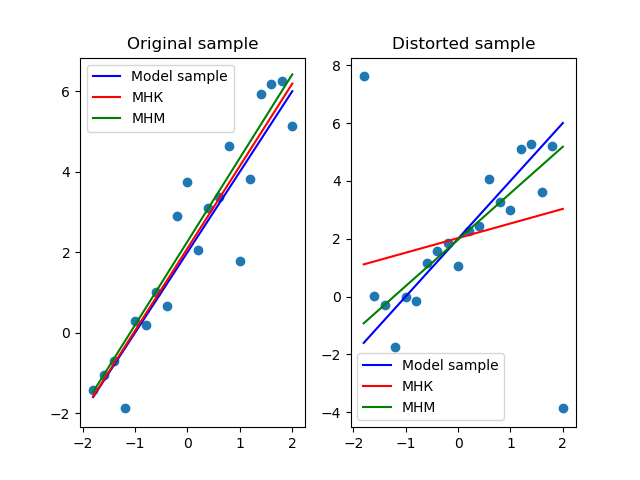
\includegraphics[scale = 0.8]{reg.png} 
    \label{fig:reg}
\end{figure}

\begin{table}[H]
\caption{Таблица оценок коэффициентов линейной регрессии без возмущёний}
\label{tab:my_label1}
\begin{center}
\vspace{5mm}
\begin{tabular}{|c|c|c|}
\hline
& $\overset{\wedge}{a}$ & $\overset{\wedge}{b}$\\
\hline
МНК &2.000&2.000\\
\hline
МНМ &2.045&2.098\\
\hline
\end{tabular}
\end{center}
\end{table}


\begin{table}[H]
\caption{Таблица оценок коэффициентов линейной регрессии с возмущёниями}
\label{tab:my_label2}
\begin{center}
\vspace{5mm}
\begin{tabular}{|c|c|c|}
\hline
& $\overset{\wedge}{a}$ & $\overset{\wedge}{b}$\\
\hline
МНК &2.000&2.000\\
\hline
МНМ &0.505 &2.023\\
\hline
\end{tabular}
\end{center}
\end{table}

\subsection{Точечная оценка параметров распределения}
\subsubsection{Метод максимального правдоподобия}

При подсчете оценок параметров закона нормального распределения методом максимального правдоподобия были получены следующие значения:
\begin{equation}
\begin{split}
    &\overset{\wedge}{m}_{\text{МП}} = -0.1235\\
   &  \overset{\wedge}{\sigma}^2_{\text{МП}} = 0.9877
\end{split}
\end{equation}
\subsubsection{Критерий Пирсона}
\begin{table}[H]
\caption{Таблица вычислений $\chi^2$}
\label{tab:my_label1}
\begin{center}
\vspace{5mm}
\begin{tabular}{|c|c|c|c|c|c|c|}
\hline
 i & $\Delta_i$ & $n_i$ & $p_i$ & $np_i$ & $n_i-np_i$ & $\frac{(n_i-np_i)^2}{np_i}$\\
\hline
1&	 $(-\infty, -1.6605]$ &	5  &	 0.0517	& 5.1670 &	 -0.1670 &	 0.0054\\
\hline
2&	(-1.6605, -0.7749)&	17&	 0.1950&	 19.4966&	 -2.4966&	 0.3197\\
\hline
3& (-0.7749, 0.1108)&	40&	 0.3390&	 33.8962& 6.1038&	 1.0991\\
\hline
4&	(0.1108, 0.9965)&	27&	 0.2778&	 27.7824&	 -0.7824&	 0.0220\\
\hline
5& $(0.9965, \infty)$&	11&	 0.1284&	 12.8411&	 -1.8411&	 0.2640\\
\hline
$\sum$&&		100&	1&	100&0&1.8665	\\

\hline
\end{tabular}
\end{center}
\end{table}

$$\chi_B^2= 1.8665$$

\subsection{Интервальные оценки параметров распределения}

\begin{table}[H]
\caption{Результаты}
\label{tab:my_label1}
\begin{center}
\vspace{5mm}
\begin{tabular}{|c|c|c|c|}
\hline
Метод & $n$&$\mu$&$\sigma$\\
\hline
&$20$&	$[-0.33527, 0.40768]$&		$[0.71165, 1.36749]$ \\
\cline{2-4}
\raisebox{1.5ex}[0cm][0cm]{На основе ММП}&100&	$[-0.20017, 0.16315]$&		$[0.79980, 1.05748]$\\
\hline
&20&	$[-0.37421, 0.44662]$&		$[0.75586, 1.11704]$ \\
\cline{2-4}
\raisebox{1.5ex}[0cm][0cm]{Асимптотический}&100	&$[-0.19705, 0.16003]$&	$[0.80188, 1.01998]$\\
\hline
\end{tabular}
\end{center}
\end{table}



\section{Выводы}
\subsection{Вычисление коэффициента корреляции}
По таблицам \ref{tab:my_label1_1}, \ref{tab:my_label1_2}, \ref{tab:my_label3}, \ref{tab:my_label4}, видно, что, при увеличении объёма выборки, подсчитанные коэффициенты корреляции стремятся к теоретическим.

Ближе всех к данному коэффициенту корреляции находится коэффициент Пирсона.

По графикам видно, что при уменьшении корреляции эллипс равновероятности стремится к окружности, а при увеличении растягивается.

\subsection{Оценки линий регрессии}
По графику \ref{fig:reg} видно, что оба метода дают хорошую оценку коэффициентов линейной регрессии, если нет выбросов. Однако выбросы сильно влияют на оценки по МНК.

Выбросы мало влияют на оценку по МНМ. Ценой за это является б\'oльшая по сравнению с МНК сложность вычисления.

\subsection{Точечная оценка параметров распределения}
В данной работе получено значение критерия согласия Пирсона $\chi_B^2 = 1.8665.$ Табличное значение квантиля  $\chi^2_{1-\alpha}(k-1)=\chi^2_{0.95}(4) = 9,4877$ \cite{chi_quant}.

Значит $\chi_B^2 < \chi^2_{0.95}(4),$ из этого следует, что основная гипотеза $H_0$ соотносится с выборкой на уровне $\alpha = 0.05.$

\subsection{Интервальные оценки параметров распределения}

По полученным результатам видно, что оба подхода дают лучший результат на выборках большого объема. Если рассматривать результаты для выборки объема $n=20$ элементов, то видно, что интервал меньше и точнее в классической интервальной оценке.

\begin{thebibliography}{}
    \bibitem{numpy}  Модуль numpy  -  https://physics.susu.ru/vorontsov/language/numpy.html
    
    \bibitem{plotlib} 
    Модуль matplotlib - https://matplotlib.org/users/index.html
    
    \bibitem{skp}
    Модуль scipy - https://docs.scipy.org/doc/scipy/reference/
    
    
    
    \bibitem{mix}
    http://stu.sernam.ru/book\_stat3.php?id=55
    
\bibitem{5_1}
Двумерное нормальное распределение: https://en.wikipedia.org/wiki/Multivariate\_normal\_distribution
\bibitem{5_2}
Коэффициент корреляции Пирса: http://statistica.ru/theory/koeffitsient-korrelyatsii/ 
\bibitem{5_3}
Коэффициент корреляции Спирмана: 
http://economic-definition.com/Exchange\_Terminology/Koefficient\_korrelyacii\_Correlation\_coefficient\_\_eto.html
\bibitem{5_4} Квадрантный коэффициент корреляции: https://www.researchgate.net/profile/Pavel\_Smirnov8/publication/\do-316973167\_Robastnye\_metody\_i\_algoritmy\_ocenivania\_korrelacionnyh\_harakteristik\_dannyh\_na\_os\do-nove\_novyh\_vysokoeffektivnyh\_i\_bystryh\_robastnyh\_ocenok\_masstaba/links/591b019d458515695282\do-8a52/Robastnye-metody-i-algoritmy-ocenivania-korrelacionnyh-harakteristik-dannyh-na-osnove-novyh-vysokoeffektivnyh-i-bystryh-robastnyh-ocenok-masstaba.pdf\#page=81
    
    
    \bibitem{lin_reg}
    https://en.wikipedia.org/wiki/Linear\_regression

\bibitem{MNK}
http://www.cleverstudents.ru/articles/mnk.html

\bibitem{6_3}
Шевляков Г. Л. Лекции по математической статистике, 2019.

\bibitem{6_4}
Вероятностные разделы математики. Учебник для бакалавров технических направлений. //Под ред. Максимова Ю.Д. - СПб.:"Иван Федоров 2001. - 592 с.
    
    
    
\bibitem{7_2}
https://en.wikipedia.org/wiki/Pearson\%27s\_chi-squared\_test

\bibitem{chi_quant}
Таблица значений $\chi^2$ -  https://en.wikipedia.org/wiki/Student\%27s\_t-distribution

    
    

\bibitem{8_1}
https://en.wikipedia.org/wiki/Confidence\_interval

\bibitem{8_2}
https://en.wikipedia.org/wiki/Student\%27s\_t-distribution

\bibitem{8_3}
https://en.wikipedia.org/wiki/Chi-squared\_distribution

\bibitem{8_4}
Шевляков Г. Л. Лекции по математической статистике, 2019.

\end{thebibliography}

\section{Приложения}


Код отчёта:\; \url{https://github.com/MisterProper9000/MatStatLabs/blob/master/MatStatLab5/MatStatLab8.tex}

Код лаборатрной:\; \url{https://github.com/MisterProper9000/MatStatLabs/blob/master/MatStatLab5/MatStatLab8.py}

%\lstinputlisting[language=Python]{MatStatLab7.py}

\end{document}